\documentclass[11pt]{article}
\usepackage{graphicx}
\usepackage{amsmath}
\usepackage{authblk}
\usepackage[margin=1in]{geometry}
\usepackage{hyperref}
\usepackage{siunitx}

\title{A Computational Approach to Maximal Colour Perception Shift}
\author{Alex Grant}
\affil{Improbability Engineering}
\date{\today}

\begin{document}
\maketitle

\begin{abstract}
We present a computational method for identifying surround colours that cause the greatest perceptual shift in the appearance of a fixed stimulus colour. The method simulates perceptual colour appearance using the CIECAM02 colour appearance model and quantifies differences in appearance via the $\Delta E_{CAM02-UCS}$ metric. By comparing the perceived colour of a fixed stimulus across a large set of candidate surrounds, we identify surrounds that maximize the perceptual shift in appearance. This system offers an automated, quantitative analogue to the explorations of contextual colour interaction pioneered by Josef Albers.
\end{abstract}

\section{Introduction}

The perceived colour of a stimulus is not determined solely by its physical properties but is deeply influenced by its surrounding context, a visual artefact due to human three-cone colour detection in the eye and subsequent neurological processing. This phenomenon is central to a wide array of optical illusions and artistic practice, notably in the pedagogical experiments of Josef Albers~\cite{albers}. In this work, we develop a \emph{computational} approach to quantify and optimize such context-driven perceptual shifts. The goal is to produce ``Albers-extrema'' by identifying candidate surround colours that most dramatically alter the perceived appearance of a fixed stimulus colour, compared to when viewed on a given surround.

\section{Colour Appearance and Perceptual Difference Metrics}

Human perception of colour differences is not linear in most common colour spaces such as sRGB or CIE 1931 XYZ~\cite{cam02}. That is, equal distances in these spaces do not correspond to equal perceptual differences. A \textit{perceptually uniform space} is one in which the geometric distance between two colour vectors approximates the perceived difference between them. Use of such colour spaces allows us to use the Euclidean distance metric to meaningfully compare perceptual shifts.

To model how a stimulus colour appears under various surrounds, we employ the CIECAM02 colour appearance model. CIECAM02 accounts for contextual influences such as luminance level, surround adaptation, and background colour. Each colour is represented in terms of perceptual attributes: lightness $J$ (perceived brightness of a colour relative to a reference white.), colourfulness $M$ (perceived intensity or saturation of colour compared to a reference grey), hue angle $h$ (describing the type of colour sensation e.g., red, blue, green).

To compare colours perceptually, we transform CIECAM02 outputs into the CAM02-UCS (Uniform Colour Space), a modification of CIECAM02 that is approximately perceptually uniform. In this space, colours are represented as coordinates $(J', a', b')$ where $J'$ is lightness, $a'$ is the red–green opponent dimension, and $b'$ is the yellow–blue opponent dimension. The perceived difference between two colours can then be computed using the Euclidean distance:

\begin{equation}
\Delta E = \sqrt{(J'_1 - J'_2)^2 + (a'_1 - a'_2)^2 + (b'_1 - b'_2)^2}
\end{equation}

This $\Delta E$ value serves as a quantitative proxy for how different two colours \emph{appear} to a human observer.

\section{Methodology}

Given a fixed stimulus colour $C_{\text{stim}}$ and an initial surround colour $C_{\text{init}}$, we compute the perceived appearance $P_{\text{init}}$ of the stimulus using CIECAM02. We then search a discretized set of surround colours $\{C_i\}$ to find candidates that, when used as the surround, produces a perceived stimulus colour $P_i$ that maximizes:

\begin{equation}
\Delta E_i = \|P_i - P_{\text{init}}\|_{\text{CAM02-UCS}}
\end{equation}

This approach keeps the physical stimulus colour constant and varies only the surround. Candidate surround $i$ is evaluated by:
\begin{enumerate}
    \item Applying it as the surround context for the stimulus colour.
    \item Computing the new perceived appearance $P_i$ of the stimulus using CIECAM02.
    \item Measuring the perceptual shift $\Delta E_i$ from the original perceived appearance $P_{\text{init}}$.
\end{enumerate}

To simulate the effect of the surround on the stimulus, we define a mapping from the stimulus colour and the surround to the perceived appearance using a simplified centre-surround model. This model assumes a uniform surround field and computes the adapted appearance of the stimulus via the chromatic adaptation and viewing condition parameters defined in CIECAM02. By modifying the surround input, the CIECAM02 model yields a different perceived output for the same  stimulus.

Surrounds with the largest $\Delta E_i$ are selected as maximally perception-shifting surrounds.

\section{Implementation}
We implemented the algorithm in Python using the \texttt{colour-science} package~\cite{colour} to handle colour space conversions and appearance modelling. Candidate surrounds are sampled from a uniform grid in sRGB space, and invalid or out-of-gamut colours are excluded. The interface allows users to input a stimulus and reference surround, compute the perceptual reference, and search for the most shifting surrounds.

To improve the clarity of results and usability of the tool, we added an optinal  perceptual similarity filter that allows users to exclude candidate surrounds with perceptual differences below a chosen threshold $\Delta E$. This ensures that only perceptually distinct results are considered in the search for maximally shifting surrounds.

The application also has the ability to search for the surround that induces the maximal perception shift in a given stimulus colour, and to search for stimulus colours that are most sensitive to perception shift when placed on a given surround.

Source code for the application can be found on github~\cite{colourshift}.

\section{Examples}

Below are example outputs generated by the program, illustrating the perceptual shift of a stimulus colour under various computed surround conditions:

\begin{figure}[h!]
\centering

\includegraphics[width=0.8\textwidth]{1.png}
\caption{Example output 1: stimulus colour and original vs maximally shifting surround.}
\end{figure}

\begin{figure}[h!]
\centering

\includegraphics[width=0.8\textwidth]{2.png}
\caption{Example output 2: second ranked alternate surround.}
\end{figure}

\begin{figure}[h!]
\centering

\includegraphics[width=0.8\textwidth]{3.png}
\caption{Example output 3: third ranked alternate surround.}
\end{figure}

\begin{figure}[h!]
\centering
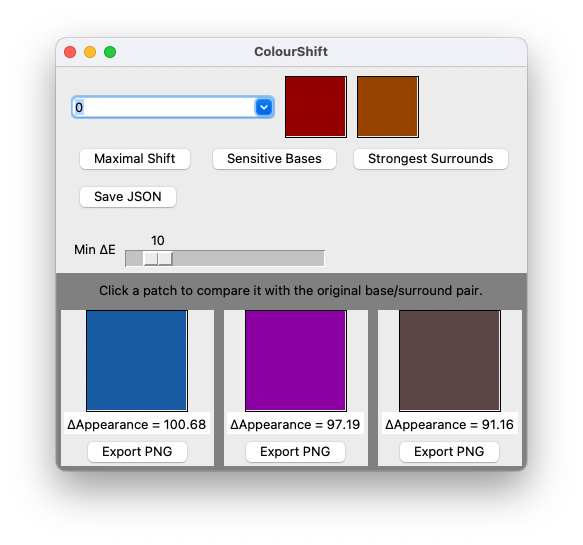
\includegraphics[width=0.8\textwidth]{screenshot.png}
\caption{Screenshot of the application interface showing stimulus, candidate surrounds, and calculated perceptual shifts.}
\end{figure}

\section{Discussion and Applications}

This method formalizes a long-standing artistic practice and extends it into quantitative territory. The results can support colour design, accessibility considerations, and educational visualization of colour relativity. Initial experiments indicate that cadidate surrounds inducing the greatest perceptual shifts often exhibit complementary hue relationships. In future work, we will investigate the structure of perceptual extrema vectors, to see if there are any compact descriptions of these sets of vectors (e.g. do they obey a particular relative relationship with respect to each other and the stimulus).

\section{Conclusion}

We introduced and implemented a computational method to identify surround colours that cause maximal perceptual change to a fixed stimulus colour. By leveraging colour appearance models and perceptual difference metrics, we provide a tool for systematically exploring contextual colour phenomena in both scientific and creative settings.

\appendix
\section{Mathematical Formulation of the Centre-Surround Model}

To estimate the perceived colour of a  stimulus $C_{\text{stim}}$ when presented against a surround $C_{\text{surr}}$, we model the visual response using the chromatic adaptation transform (CAT) within CIECAM02. Specifically, we compute the appearance of the stimulus as it would be perceived in a viewing condition modified by the surround.

Let $XYZ_{\text{stim}}$ and $XYZ_{\text{surr}}$ be the tristimulus values of the stimulus and surround in CIE 1931 XYZ coordinates, where $Y$ represents luminance, and $X$ and $Z$ are derived from the human eye's cone response curves. The steps are as follows:

\begin{enumerate}
  \item Compute the adapting field luminance $L_A$ and surround factor $F$ as a function of $C_{\text{surr}}$.
  \item Define a white point reference from $C_{\text{surr}}$ (or an average of surround field) to be used for the chromatic adaptation.
  \item Apply the chromatic adaptation transform (e.g., CAT02) to $XYZ_{\text{stim}}$ using the computed white point.
  \item Run the full CIECAM02 forward model on the adapted $XYZ_{\text{stim}}$ to obtain perceptual attributes $(J, M, h)$.
  \item Convert $(J, M, h)$ to CAM02-UCS $(J', a', b')$ coordinates.
\end{enumerate}

In practice, we use the \texttt{colour-science} implementation to perform these transformations. The key idea is that the surround modifies the parameters of the visual environment, thereby altering the chromatic adaptation state and changing the perceived appearance of the stimulus.

\bibliographystyle{plain}
\begin{thebibliography}{9}
\bibitem{colourshift}
Alex Grant,
\texttt{colourshift} Python package, 
\url{https://github.com/grantaj/colourshift}

\bibitem{albers}
Josef Albers,
\textit{Interaction of Color},
Yale University Press, 1963.

\bibitem{cam02}
Mark D. Fairchild,
\textit{Color Appearance Models},
Wiley, 3rd Edition, 2013.

\bibitem{colour}
Mansencal, Thomas et al.,
\texttt{colour-science} Python package,
\url{https://github.com/colour-science/colour}
\end{thebibliography}

\end{document}
